%%%%%%%%%%%%%%%%%%%%%%%%%%%%%%%%%%%%%%%%%%%%%%%%%%%%%%%%%%%%%%%%%%%%%%%%%%%%
%% Author template for INFORMS 2023 BSS Data Challenge Competition
%% -- based on Author template for Operations Research (informs3.cls)
%%%%%%%%%%%%%%%%%%%%%%%%%%%%%%%%%%%%%%%%%%%%%%%%%%%%%%%%%%%%%%%%%%%%%%%%%%%%
\documentclass[competition,nonblindrev]{informs3-competition} 

\DoubleSpacedXI % Made default 4/4/2014 at request
%%\OneAndAHalfSpacedXI % current default line spacing
%%\OneAndAHalfSpacedXII
%%\DoubleSpacedXII
%\usepackage[numbers]{natbib}
%\usepackage[natbib=true, style=authoryear]{biblatex}
% \usepackage{endnotes}
% \let\footnote=\endnote
% \let\enotesize=\normalsize
% \def\notesname{Endnotes}%
% \def\makeenmark{$^{\theenmark}$}
% \def\enoteformat{\rightskip0pt\leftskip0pt\parindent=1.75em
%   \leavevmode\llap{\theenmark.\enskip}}
%\usepackage{booktabs}
%\usepackage[font=small]{caption}%
%\usepackage[size=small]{subcaption}
\TheoremsNumberedThrough     % Preferred (Theorem 1, Lemma 1, Theorem 2)
%\TheoremsNumberedByChapter  % (Theorem 1.1, Lemma 1.1, Theorem 1.2)
\ECRepeatTheorems

%% Setup of the equation numbering system. Outcomment only one.
%% Preferred default is the first option.
\EquationsNumberedThrough    % Default: (1), (2), ...
%\EquationsNumberedBySection % (1.1), (1.2), ...


%%%%%%%%%%%%%%%%
\usepackage[subtle]{savetrees}
\let\FigureCaptionFontStyle\undefined
\def\FigureCaptionFontStyle{\mdseries}
\begin{document}
%%%%%%%%%%%%%%%%
% Corresponding author's name for the running heads
\RUNAUTHOR{Jie Wang}

% Title or shortened title suitable for running heads. Sample:
% \RUNTITLE{Bundling Information Goods of Decreasing Value}
% Enter the (shortened) title:
\RUNTITLE{Distributionally Robust Offline Pricing}

\TITLE{Reliable Offline Pricing in eCommerce: A Distributionally Robust Viewpoint}

% Corresponding author or team lead. A single point of contact for each team submission is requested. 
\ARTICLEAUTHORS{
\AUTHOR{Jie Wang}
\AFF{School of Industrial and Systems Engineering, Georgia Institute of Technology, Atlanta, GA 30332, \EMAIL{jwang3163@gatech.edu}}
}

\ABSTRACT{You should replace this sentence with your abstract that quickly summarizes your approach and findings.}



\maketitle
%%%%%%%%%%%%%%%%%%%%%%%%%%%%%%%%%%%%%%%%%%%%%%%%%%%%%%%%%%%%%%%%%%%%%%

\section{Introduction}

In the introduction, you should include an overview of the approach. Throughout the document include citations as appropriate. As an example, include citations of the form: (BSS, 2023) or BSS (2023). Included figures and tables should be labeled and captioned with a short description.



\section{Problem Setup}
Consider a retailer who sells a single product with finite amount of inventory.
Assume the amount of inventory available for sale, denoted as $y\in\mathbb{R}_+$ is known to the retailer, and he/her determines the price $p\in[p^l, p^u]$ for sale.
%an unit price $p\in[p^l, p^u]$ for each product to sale.
Besides, the retailer is provided with the competitors' selling information $z\in \mathbb{R}^{M}$ with $M\in\mathbb{N}_+$, which can be viewed as a covariate variable.
Here we assume that both the price decision $p$ and the covariate $z$ will influence the distribution of the customer demand $D$, which follows the probability distribution $f_D(p, z)$.
%demand distribution, denoted as $D\sim f_D(p, z)$.
The goal is to select the optimal price such that the expected profit $\mathbb{E}_{D\sim f_D(p,z)}[c(p,D)]$ is maximized.
In the following, we provide the detailed expression regarding the loss function $c(p,D)$.

\noindent{\bf Loss Model.}
%\paragraph{Loss Model.}
It is known that the profit depends on \emph{sales}, \emph{Cost of Goods Sold}~(COGs), \emph{eCommerce Fee}~(FBA), \emph{Referral Fee}~(REFFEE), and \emph{Ad Spend}~(ADSPEND). 
Given the price $p$, customer demand $D$, and inventory level $y$, we know $\mathrm{sales}=p(D\land y)$.
We make the following assumption regarding the other four factors:
\begin{assumption}\label{Assumption:model}
\begin{enumerate}
    \item 
$\mathrm{COGs} = a_1\cdot(D\land y)$.
    \item
$\mathrm{FBA} = a_2\cdot(D\land y)$.
    \item
$\mathrm{REFFEE} =15\%\cdot p(D\land y)$.
     \item
$\mathrm{ADSPEND}$ is a constant independent of any variable.
\end{enumerate}
\end{assumption}
Here we validate these assumptions using the provided SKU dataset \textsf{File Folders SKU 21} and it turns out that these models fit the data with high confidence level.
Specifically, the coefficients $a_1=4.43965609, a_2=6.60097822$.
Based on Assumption~\ref{Assumption:model}, we re-write the loss function $c(p,D)=0.85\cdot p(D\land y) - (a_1+a_2)\cdot (D\land y) - \mathrm{ADSPEND}$.
Therefore, the profit maximization problem with known demand distribution becomes
\begin{equation}\label{Eq:true:loss}
\max_{p\in[p^l, p^u]}~\mathbb{E}_{D\sim f_D(p,z)}\Big[ 
0.85\cdot p(D\land y) - (a_1+a_2)\cdot (D\land y) 
\Big] - \mathrm{ADSPEND}
\end{equation}
In practice, we assume the inventory level $y$, covariate (i.e., competitors' prices) $z$, and constant $\mathrm{ADSPEND}$ are given.
For example, with the given dataset, one can estimate $y, z, \mathrm{ADSPEND}$ based on time series prediction using historical data.
From the plot in Figure~\ref{fig:adspend}, we find the variable $\mathrm{ADSPEND}$ seems to be correlated with $\mathrm{unitsordered}$.
So we predict the future value of $\mathrm{ADSPEND}$ based on historical data of $\mathrm{ADSPEND}$ and $\mathrm{unitsordered}$ jointly.
\begin{figure}[t]
    \centering
    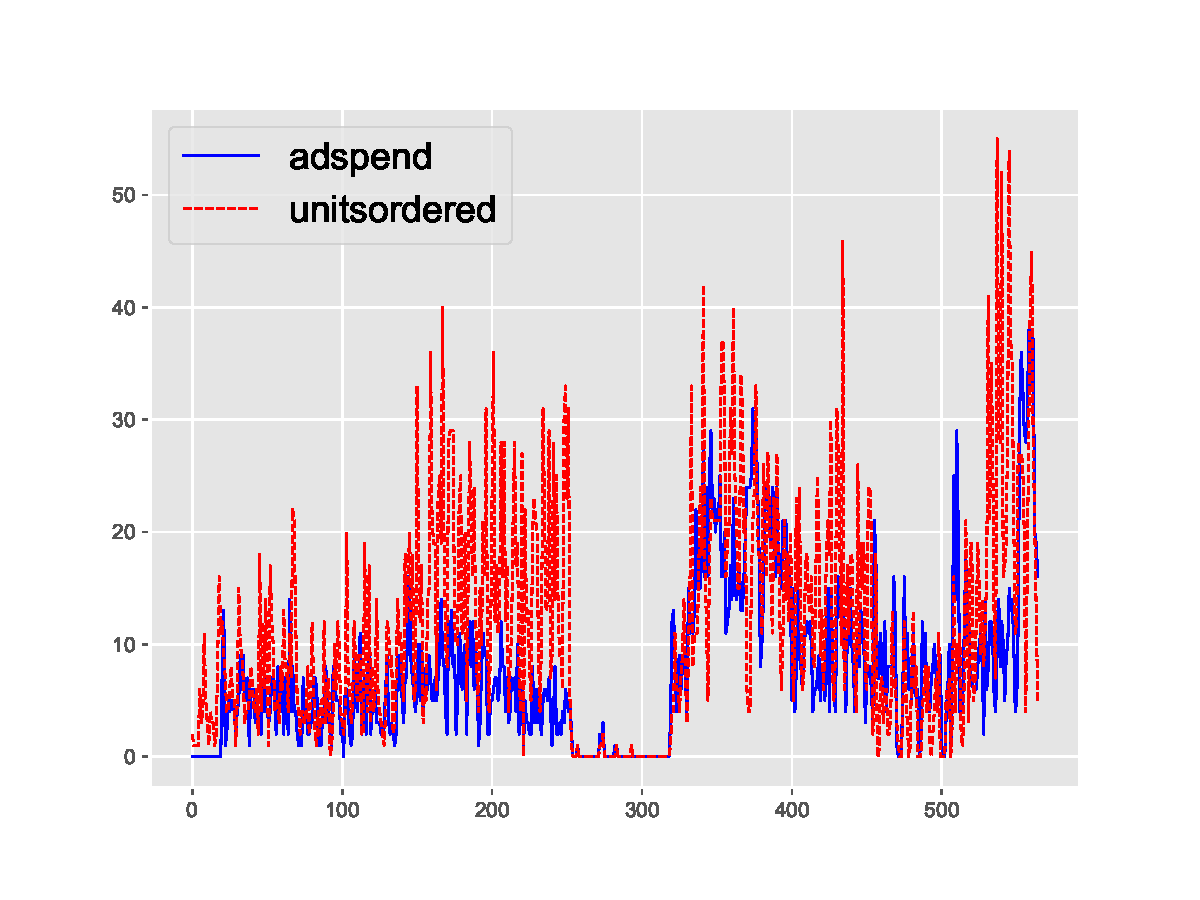
\includegraphics[width=0.5\textwidth]{adspend_units.pdf}
    \caption{Plot of adspend and units of order versus time index}
    \label{fig:adspend}
\end{figure}
However, the demand distribution $f_D(p,z)$ is usually not available.
In the following, we provide a non-parametric and data-driven way for estimating $f_D(p,z)$ based on the collected data.

\noindent 
{\bf Demand Distribution.}
We provide a data-driven estimation of the demand distribution $f_D(p,z)$, in which only data samples $\{(p^i, z^i, D^i)\}_{i=1}^N$ are available. 
For a given price-covariate pair $(p,z)$, we approximate the true demand distribution using the weighted discrete distribution sharing the same support of the training dataset:
\[
\widehat{\mathbb{P}}_n^{(p,z)} = \sum_{i=1}^N\omega^i(p,z)\delta_{D^i},
\]
where the weight function $\{\omega^i(p,z)\}_{i=1}^N$ are obtained using the (Gaussian) kernel regression model:
\[
\omega^i(p,z)\propto \exp\left( 
\frac{-\|(p,z) - (p^i,z^i)\|_2^2}{2\sigma^2}
\right),\quad 
\sum_{i=1}^N\omega^i(p,z)=1.
\]
%$k$-nearest neighbor model.
%random forest model following techniques from the existing literature~\citep{bertsimas2020predictive}.
Previous studies have proposed several modeling for the customer demand, such as additive model~\cite{biswas2018price}, \cite{wang2015optimal}, multiplicative model~\cite{kazaz2015price}, \cite{salinger2011simple}, and linear model~\cite{bu2022context}. However, it is vague whether those models result in accurate estimation of the demand in our setting because the covariate $z$ is involved. 
Instead we use a data-driven estimator in this part, which is quite flexible as we "let the data speak for itself".


\noindent 
{\bf Distributionally Robust Formulation.}
A natural idea is to solve the sample average approximation~(SAA) counterpart of problem~\eqref{Eq:true:loss}, i.e., by replacing $f_D(p,z)$ with the estimated distribution $\widehat{\mathbb{P}}_n$ and solve the approximated problem.
However, the SAA problem may not achieve satisfactory performance because the distributional estimate $\widehat{\mathbb{P}}_n$ is not accurate enough.
Instead, we consider solving the distributionally robust counterpart of the SAA problem using the %KL-divergence 
$2$-Wasserstein distance
to model the ambiguity set:
\[
\max_{p\in[p^l, p^u]}~\left\{\min_{ \mathbb{P}:~\mathrm{supp}(\mathbb{P})\subseteq \mathrm{supp}(\widehat{\mathbb{P}}_n^{(p,z)})}~\mathbb{E}_{D\sim \mathbb{P}}[c(p,D)]:~
\mathcal{W}\left(\mathbb{P},\widehat{\mathbb{P}}_n^{(p,z)}\right)\le \epsilon
\right\}.
\]
For fixed price $p$ and covariate $z$, the inner minimization problem can be reformulated as a linear program:
\[
\begin{aligned}
\min_{\gamma\in\mathbb{R}^{N\times N}, \nu\in\mathbb{R}^N_+}&\quad 
\sum_{i=1}^N\nu_ic(p, D^i)\\
\mbox{s.t.}&\quad \sum_{i=1}^N\gamma_{i,j}=\nu_j, \sum_{j=1}^N\gamma_{i,j}=\omega^i(p,z)\\
&\quad \sum_{i,j=1}^N\gamma_{i,j}|D^i - D^j|^2\le \epsilon^2.
\end{aligned}
\]



\subsection{Results}
One piece of evidence can be any numerical results you have that justify your methodology.

\section{Conclusion}

Provide a summary of key findings.

\section{Team Member(s)}

%List all team members associated with the submission, including the corresponding author. A team’s solution should be submitted once (as opposed to each member of the team submitting the same solution individually).

\begin{itemize}
\item Jie Wang, Georgia Institute of Technology, Atlanta, GA 30332, jwang3163@gatech.edu
%\item Team Member 2, Affiliation and address, TM2@email.com
%\item Team Member 3, Affiliation and address, TM3@email.com
\end{itemize}




% References here (outcomment the appropriate case)

% CASE 1: BiBTeX used to constantly update the references
%   (while the paper is being written).
%\bibliographystyle{ormsv080} % outcomment this and next line in Case 1
%\bibliography{<your bib file(s)>} % if more than one, comma separated

% CASE 2: BiBTeX used to generate mypaper.bbl (to be further fine tuned)
%\input{mypaper.bbl} % outcomment this line in Case 2

%If you don't use BiBTex, you can manually itemize references as shown below.

\bibliographystyle{informs2014} 
{
\footnotesize
\bibliography{shortbib}
}


%%%%%%%%%%%%%%%%%
\end{document}
%%%%%%%%%%%%%%%%%
